\section{Baryons}
A baryon is a subatomic particle. It is composite and contains three quarks.
The baryons form together with the mesons the class of the hadrons. Mesons are 
composed of two quarks, one quark and one antii-quark.\\
Protons and neutrons which are the components of our normal matter are baryons. 
These are the lightest baryons. The proton is made of two up quarks and one down 
quark. The neutron contains two down quarks and one up quark.\\
All observed events so far feature that the number of baryons in a reaction is 
observed. To use this in calculations every quark get the baryon number \(B = 1/3\) and 
every anti-quark \(B = -1/3\). In a decay from a baryon (\(\sum B = 1\)) the final 
products has to be a baryon (\(\sum B = 1\)) or two baryons (\(\sum B = 2\)) 
and an anti-baryon (\(\sum B = -1\)) and so on. 

\subsection{\(\Lambda_c^+\) Baryon}
The \(\Lambda_c^+\) has a mass of \(2286.46 \pm 0.14 \text{MeV}^
{\text{\cite{lambda-pdg}}}\) and a mean life time of \(\left( 2.00 \pm 0.06\right)
\cdot 10^{-13} \text{s}^{\text{\cite{lambda-pdg}}}\). It is one of the lightest charmed 
baryons and is made of one up, down and charm quark. Its charge is +1 of the 
elementary charge\(^{\text{\cite{lambda-pdg}}}\).

\section{Decays}
Decays are processes with one particle in the initial state and n particles 
in the final state for n= 2,3,{\ldots}. The decayed particle must not be in the final 
state. This makes the difference to radiation processes. The decay process can 
always be transformed in to the rest mass frame of the decayer. So the mass 
of the particle in the inital state is a limit for the dynamic of the process.\\
A decay process or more general a transition process is characterized through 
Fermi's golden rule:
\begin{equation}
  \Gamma_{fi} = 2 \pi |T_{fi}|^2 \rho\left(E_i\right), \label{eq:fermi}
\end{equation}
where \(T_{fi}\) is the transition matrix element and 
\(\rho\left(E_i\right)\) is the density of states. The result is the transition 
rate \(\Gamma_{fi}\). In natural units the unit of the transition rate is \(\text{GeV}^{-1}\).\\
The \(\Gamma_{fi}\) is also called partial decay width. And is characteristic value 
of a decay process. The sum over all partial decay widths is called 
total decay width:
\begin{equation}
  \Gamma_i = \sum_f \Gamma_{fi}. \label{eq:total}
\end{equation}
The total width{\eqref{eq:total}} is an criterion for the lifetime of the 
decaying particle. The lifetime  of the particle in natural units is the 
inverse of \(\Gamma_i\):
\begin{equation}
  \tau_i = \frac{1}{\Gamma_i}. \label{eq:lifetime}
\end{equation}
The branching ratio is the probability to decay in a specific final 
state. It can be calculated with the partial and total decay width:
\begin{equation}
  BR( i \rightarrow f) = \frac{\Gamma_f}{\Gamma}. \label{eq:br}
\end{equation}

\section{Weak Decay}
A weak decay is the transition of a particle through the weak interaction. An 
elementary particle that is possibly part of an composite can in this 
way decay to a W\(^\pm\)-Boson and a correspondending particle. But the W-Boson only 
couple to lef-handed fundamental partciles and right-handed fundamental 
anti-particles. The spinor for the weak interaction than looks like 
{\eqref{eq:spinor}}. There the upper particle have isospin -1/2 and the lower isospin 
+1/2.
\begin{equation}
  \Spvek{\nu_e; e^-}_L,\Spvek{\nu_\mu; \mu^-}_L, \Spvek{s; c}_L, \Spvek{e^+; \bar{\nu}_e}_R, 
  \Spvek{\mu^+; \bar{\nu}_\mu}_R \text{ etc.} \label{eq:spinor}
\end{equation}
Above only the particles are shown that are relevant for this 
thesis.

\begin{figure}[h]
  \centering
  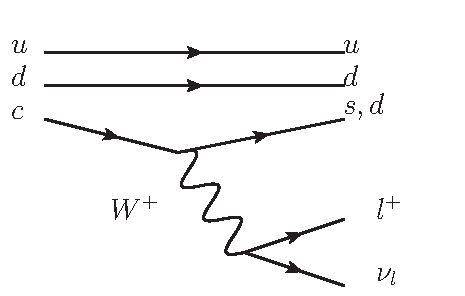
\includegraphics[page=1, width=0.5\textwidth]{semileptonic_lambdac+}
  \caption{Semileptonic decay modes of the \(\Lambda_c^+\) into a neutron (udd)
    or a \(\Lambda\) (uds), an positron or an anti-muon and the correspondending 
  neutrino (own graphic)}\label{fey:lambda}
\end{figure}

In the Feynman diagram {\ref{fey:lambda}} the semileptonic decay of a \(\Lambda_c^+\) 
is visible. The up and down quark from the \(\Lambda_c^+\) are unchanged. 
They can only influence the transition matrix element through a different 
behavior of the charm quark. The charm quark transforms through the weak 
decay in to a down or strange quark. The down quark forms with the other two 
qarks a neutron and the strange quark a \(\Lambda\). The emited W\(^+\)-Boson 
decays leptonic in an anti-lepton and the correspondending neutrino.
Other decays of the W\(^+\)-boson are possible. For this thesis only the 
semileptonic decays channels are relevant. The complete dynamic of the process 
will be discussed in {\ref{sec:v-a}}. In this section we will take a closer 
look at the W\(^\pm\) propagator.\\
The value for a W\(^\pm\) propagator is \(\frac{g_w^2}{8}\frac{1}{q^2 - m_W^2}\).
The transferred momentum is \(q^2 = \left(p_f - p_i\right)^2\). It is limited 
by the initial state mass and for most decays this is much less than the mass 
of the W\(^\pm\) boson. The last fraction can be approximated through 
\(-\frac{1}{m_W^2}\) for \(m_i \ll m_W\). The whole term becomes to \(-\frac{g_w^2}{8 m_W^2}\) 
and this is the Fermi coupling constant \(G_F\) except a factor \(-\frac{1}{sqrt{2}}\):
\begin{equation}
  \frac{G_F}{\sqrt{2}} = \frac{g_w^2}{8 m_W^2}. \nonumber
\end{equation}
The weak decay has in this approximation a threesome vertex with the coupling 
constant \(G_F\).

\section{V-A current} \label{sec:v-a}
The value of a vertex where two matching leptons transforms into a  
W\(^\pm\) boson is \(-i \frac{g}{2\sqrt{2}} \gamma^\mu\left(1-\gamma^5\right)\).
If the sum is splitted, the the term without \(\gamma^5\) is called vector and 
the part with the \(\gamma^5\) axial-vector through the geometrical effect of 
the \(\gamma\)-matrix. The transition from quarks needs an additional factor 
\(V_{if}\). i is the quark and in the initial state and f the quark in the 
final state. The factor comes from the CKM-matrix\(^{\text{\cite{ckm}}}\). The 
matrix from {\cite{ckm}} is
\begin{equation}
  V_{CKM} =
  \begin{bmatrix}
    0.97434^{+0.00011}_{-0.00012} &  0.22506 \pm 0.00050 & 0.00357 \pm 0.00015 \\
    0.22492 \pm 0.00050 & 0.97351 \pm 0.00013 & 0.0411 \pm 0.0013 \\
    0.00875^{+0.00032}_{-0.00033} & 0.0403 \pm 0.0013 & 0.99915 \pm 0.00005
  \end{bmatrix}. \label{eq:ckm}
\end{equation}
With the general Feynman rules for vertices and propagators the transition matrix 
element becomes to
\begin{equation}
  T = \frac{G_F}{\sqrt{2}} V_{Qq} \bar{u_l}\gamma^\mu\left(1 - \gamma^5\right) 
  u_{\nu_l} \langle B(p', s') | J_\mu | \Lambda_c(p, s) \rangle \label{eq:trans}
\end{equation}
ike in {\cite[Eq. 1]{Frank}}, where B in stands for the neutron or \(\Lambda\). The current 
\(J_\mu\) can be splitted in a vector and an axial-vector part \(J_\mu = V_\mu - 
A_\mu \) like in
\begin{align}
  \langle B(p', s') | V_\mu | \Lambda_c(p, s) \rangle & = \bar{u}(p', s') 
  \left( F_1(q^2) \gamma_\mu + F_2(q^2)\frac{p_\mu}{m_{\Lambda_c}} + 
  F_3(q^2)\frac{p'_\mu}{m_B} \right) u(p, s) \nonumber \\
  \langle B(p', s') | A_\mu | \Lambda_c(p, s) \rangle & = \bar{u}(p', s') 
  \left( G_1(q^2) \gamma_\mu + G_2(q^2)\frac{p_\mu}{m_{\Lambda_c}} + 
  G_3(q^2)\frac{p'_\mu}{m_B} \right) \gamma^5 u(p, s). \label{eq:v-a}
\end{align}
The \(F_i\) and \(G_i\) are the form factors for the transition. They are specific 
for the initial and final baryons and describe the different behavior of the 
quarks in a bound state in contrast to the free decay. The functional behavior 
of these form factors is related to \(q^2 = (p - p')^2\).

\section{Monte-Carlo methods}
The \texttt{Sherpa} software use Monte-Carlo methods to calculate the decay
widths and  randomly select the dynamics of a process. In my thesis I did 
not work on the Monte-Carlo algorithms. For details about these methods 
the diploma{\cite{diploma}} from Dr. Frank Siegert can be considered.

